%!TEX root = ../Fast_Contour_Tracing_Algorithm.tex
% -*- root: ../Fast_Contour_Tracing_Algorithm.tex -*-

\section{Analysis of Conventional Contour-following Algorithms}

% Figure \ref{fig:image8} illustrates the tracing results of pixel following methods based on the contour shown in figure \ref{fig:image1}. In the figure, the arrow with an anchor is the tracer at the starting pixel, a solid arrow shows the movement operation of the tracer, and a dotted line is the way point (detected pixel) for determining whether or not the pixel is a contour pixel for pixel following.

Figure \ref{fig:image8} illustrates the tracing results of the pixel-following methods based on the contour shown in Figure \ref{fig:image1}. In the figure, the arrow with an anchor is the tracer at the starting pixel, the solid arrow shows the movement operation of the tracer, and the dotted line is the way point (detected pixel) for determining whether or not the pixel is a contour pixel for pixel following.

%%% Image 8
\begin{figure}[htbp]
	\centering
	\subfloat[]{ 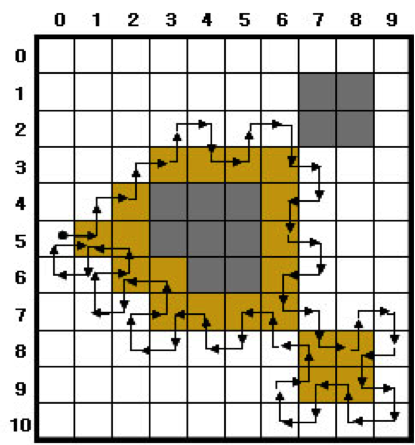
\includegraphics[width=0.33\textwidth]{3.Analysis/fig8-a.png} \label{fig:img8-a} }
	\subfloat[]{ 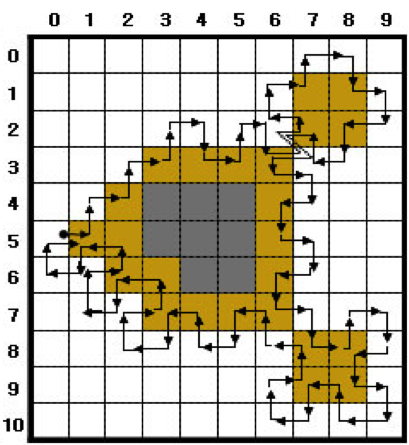
\includegraphics[width=0.33\textwidth]{3.Analysis/fig8-b.png} \label{fig:img8-b} }
	\subfloat[]{ 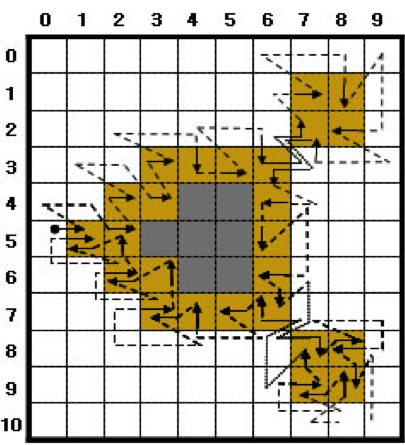
\includegraphics[width=0.33\textwidth]{3.Analysis/fig8-c.png} \label{fig:img8-c} } //
	\subfloat[]{ 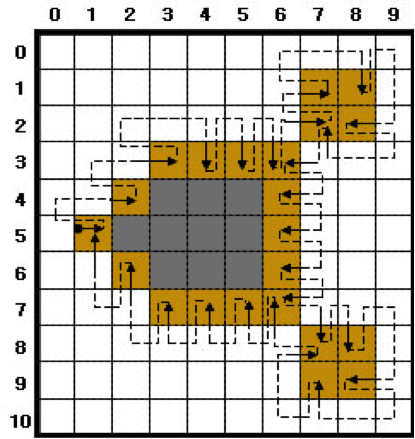
\includegraphics[width=0.33\textwidth]{3.Analysis/fig8-d.png} \label{fig:img8-d} }
	\subfloat[]{ 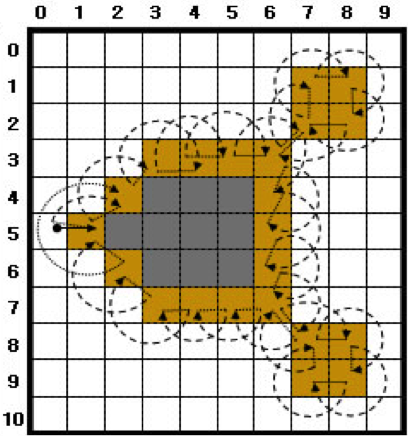
\includegraphics[width=0.33\textwidth]{3.Analysis/fig8-e.png} \label{fig:img8-e} }
	\subfloat[]{ 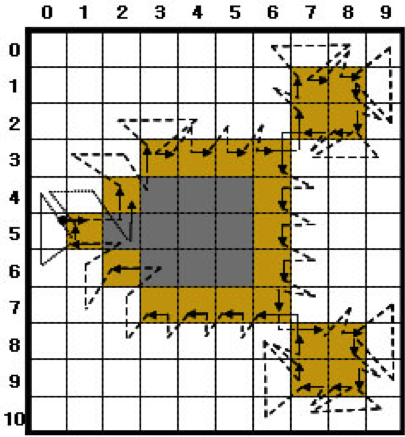
\includegraphics[width=0.33\textwidth]{3.Analysis/fig8-f.png} \label{fig:img8-f} }
	 
	\caption{Comparison of conventional contour pixel-following algorithms \protect\subref{fig:img8-a} SBF \protect\subref{fig:img8-b} MSBF \protect\subref{fig:img8-c} ISBF \protect\subref{fig:img8-d} MNT \protect\subref{fig:img8-e} RSA \protect\subref{fig:img8-f} TPA}
	\label{fig:image8}
\end{figure}

%%%%%
\subsection{Pixel-following Cases}

% As shown in figure \ref{fig:image8}, the ISBF traces most types of contour pixels such as the inner corner, outer corner, inner-outer corner, and straight-line pixels. In the case of the SBF, there are inconsistencies regarding tracing at the inner corner and inner-outer corner. For example, in the figure, the inner corner pixel (3, 6) and inner-outer corner pixel (7, 8) are traced, but the inner corner (3, 4) and inner-outer corner (7, 9) pixels are missed. In the case of the MSBF, all the inner-outer corner pixels are traced, but it has inconsistencies with regard to tracing the inner corner pixel. Moreover, the MNT, RSA, and TPA have no inconsistency problems but they cannot trace the inner corners. Among these algorithms, the TPA can be easily changed to trace an inner corner pixel since it has way points on the inner corners, as shown in figure \ref{fig:img8-f}. 

As shown in Figure \ref{fig:image8}, the ISBF traces most types of contour pixels such as the inner corner, outer corner, inner-outer corner, and straight-line pixels. In the case of the SBF, there are inconsistencies regarding tracing at the inner corner and inner-outer corner. For example, in the figure, the inner-corner pixel $(3, 6)$ and inner-outer corner pixel $(7, 8)$ are traced, but the inner corner $(3, 4)$ and inner-outer corner $(7, 9)$ pixels are missed. In the case of the MSBF, all the inner-outer corner pixels are traced, but it has inconsistencies with regard to tracing the inner-corner pixel. Moreover, the MNT, RSA, and TPA have no problems with consistency, but they cannot trace the inner corners. Among these algorithms, the TPA can be easily changed to trace an inner-corner pixel because it has waypoints on the inner corners, as shown in Figure \ref{fig:img8-f}.



%%%%%
\subsection{Start-up Condition and Stopping Criteria}

% The pixel following algorithm functions under the criteria of start and stop to avoid incompleteness of tracing and infinite tracing.
The pixel-following algorithm functions using the criteria of start-and-stop to avoid incompleteness of tracing and infinite tracing.

\subsubsection{Assumption for Start}

Commonly, start of tracing occurs when the tracer enters a black pixel from a white pixel. Due to this reason, at the start of tracing, the tracer must be placed on a black pixel and its rear pixel $P_{Rear}$ should be white. Moreover, in the case of the MSBF and ISBF, if the $P_{Left-Rear}$ of the start pixel is an inner-outer corner pixel, they cannot trace all the contour pixels by using their stopping criteria \cite{Cheong2006Advanced}. In addition, TPA has to select a start pixel that has white pixels at the tracer positions $P_{Left}$, $P_{Left-Rear}$, and $P_{Right-Rear}$\cite{Ghuneim2000Contour}; otherwise, it cannot trace the left pixel of the contour. 

Commonly, tracing starts when the tracer enters a black pixel from a white pixel. Therefore, at the start of tracing, the tracer must be placed on a black pixel and its rear pixel $P_{Rear}$ should be white. Moreover, in the case of the MSBF and ISBF, if the $P_{Left-Rear}$ of the start pixel is an inner-outer corner pixel, it cannot trace all of the contour pixels using their stopping criteria [10]. In addition, TPA has to select a start pixel that has white pixels at the tracer positions $P_{Left}$, $P_{Left-Rear}$, and $P_{Right-Rear}$ [7]; otherwise, it cannot trace the left pixel of the contour. 

\subsubsection{Stop Criterion}
% There are three methods for stopping the contour tracing \cite{Ghuneim2000Contour}. The first method is Jacob's stopping criterion \cite{Ghuneim2000Contour} that terminates the trace when the tracer reenters the start pixel with an absolute direction that is the same as the start direction, i.e., if the current tracer $T(P,d)$ is the same as the start tracer $S(P,d)$, the pixel following is terminated. The SBF, MSBF, and ISBF use this criterion and their tracing terminates at the start pixel, as shown in figures \ref{fig:img8-a}-\ref{fig:img8-c}. The second method uses the number of reentries to the start pixel. In figures \ref{fig:img8-d} and \ref{fig:img8-f}, the tracers of MNT and TPA revisit the start pixel (1, 5) with different directional information; therefore, they do not stop but go to the next contour pixel if the first method is applied. For this reason, if a specified number of reentries such as three or four times is satisfied, the trace is terminated \cite{Ghuneim2000Contour}. Sometimes, this method is not efficient because it requires unnecessary tracing to be performed one or more times. The final method checks the trace route that is traced by the previous pixel and current pixel of the tracer and determines whether or not it has already been passed. This method is used for RSA \cite{Ghuneim2000Contour,Mirante1982Radial} since its tracer has no directional information but only pixel location information. In other words, whenever the tracer enters the $i$-th contour pixel, the current pixel location $P_i$ is appended sequentially into the traced contour path. Moreover, if the traced path of $(P_{i-1}, P_i)$ appears twice, the tracing is terminated. This method can be applied for all pixel following methods and it is simpler than the second method; however, it requires more operations than Jacob's stopping criterion.

There are three methods for stopping the contour tracing \JHMEMO{[7]}. The first method is Jacob's stopping criterion \JHMEMO{[7]}, which terminates the trace when the tracer reenters the start pixel with an absolute direction that is the same as the start direction, i.e., if the current tracer $T(P,d)$ is the same as the start tracer $S(P,d)$, the pixel following is terminated. The SBF, MSBF, and ISBF use this criterion, and their tracing terminates at the start pixel, as shown in Figures \ref{fig:img8-a}-\ref{fig:img8-c}. The second method uses the number of reentries to the start pixel. In Figures \ref{fig:img8-d}-\ref{fig:img8-f}, the tracers of MNT and TPA revisit the start pixel $(1, 5)$ with different directional information; therefore, they do not stop, but rather go to the next contour pixel if the first method is applied. For this reason, if a specified number of reentries, e.g., three or four times, is satisfied, the trace is terminated \JHMEMO{[7]}. This method is sometimes not efficient because it requires unnecessary tracing to be performed one or more times. The final method checks the trace route that is traced by the previous pixel and current pixel of the tracer, and determines whether it has already been passed. This method is used for RSA [7,8] because its tracer has only pixel-location information, and no directional information. In other words, whenever the tracer enters the $i$-th contour pixel, the current pixel location $P_i$ is appended sequentially into the traced contour path. Moreover, if the traced path of $(P_{i-1}, P_i)$ appears twice, the tracing is terminated. This method can be applied for all pixel-following methods, and it is simpler than the second method; however, it requires more operations than Jacob's stopping criterion.

\subsubsection{Limitations of Conventional Pixel-following Methods}

% The abovementioned conventional pixel following methods have certain limitations. First, some of the algorithms such as SBF and MSBF perform unnecessary movement operation on a white pixel, as shown in figures \ref{fig:img8-a} and \ref{fig:img8-b}. Second, all the algorithms cannot define the contour in the case of contour pixels; therefore, they cannot be a descriptive feature of the object and determine connectivity among objects. For example, in figure \ref{fig:img8-b}, the MSBF detects (2, 7) as the inner-outer corner pixel, but does not indicate (8, 7) as an inner-outer corner because the traced paths on the pixels are different. Moreover, the MSBF also cannot determine the inner corner, outer corner, and straight line pixel like the SBF does. In case of the ISBF, it determines the inner-outer corner, front inner corner, and front straight line pixels but cannot determine the left inner corner, left straight line and some of the outer corner pixels, as shown in figure \ref{fig:img8-c}. Similarly, MNT and RSA cannot determine and detect the inner corners, and TPA cannot classify the contour pixels into the different types of contour pixels. Finally, the data size of the traced contour must be considered. The pixel following methods save all the pixel points; therefore, their data are larger than those of the RD code method.

The abovementioned conventional pixel-following methods have certain limitations. First, some of the algorithms, such as SBF and MSBF, perform unnecessary movement operations on white pixels, as shown in Figures \ref{fig:img8-a} and \ref{fig:img8-b}. Second, not all of the algorithms can define the contour in the case of contour pixels; therefore, they cannot be a descriptive feature of the object and determine connectivity among objects. For example, in Figure \ref{fig:img8-b}, the MSBF detects $(2, 7)$ as the inner-outer corner pixel, but does not indicate $(8, 7)$ as an inner-outer corner because the traced paths on the pixels are different. Moreover, the MSBF also cannot determine the inner corner, outer corner, and straight-line pixel, as is the case with the SBF. In the case of the ISBF, it determines the inner-outer corner, front-inner corner, and front-straight line pixels, but cannot determine the left-inner corner, left-straight line, and some of the outer-corner pixels, as shown in Figure \ref{fig:img8-c}. Similarly, MNT and RSA cannot determine and detect the inner corners, and TPA cannot classify the contour pixels into the different types of contour pixels. Finally, the data size of the traced contour must be considered. The pixel-following methods save all the pixel points; therefore, their data are larger than those of the RD code method.


